%%%%%%%%%%%%%%%%%%%%%%%%%%%%%%%%%%%%%%%%%%%%%%%%%%%%%%%%%%%%%%%%%%%%%%%%%%%%%%%%%%
\begin{frame}[fragile]\frametitle{}
\begin{center}
{\Large Background}
\end{center}
\end{frame}


%%%%%%%%%%%%%%%%%%%%%%%%%%%%%%%%%%%%%%%%%%%%%%%%%%%%%%%%%%%
\begin{frame}[fragile]\frametitle{New Programming Language?}

\begin{center}

\includegraphics[width=0.8\linewidth,keepaspectratio]{promptengg1}

{\tiny (Ref: Prompt Engineering Sudalai Rajkumar)}

\end{center}				

\end{frame}


%%%%%%%%%%%%%%%%%%%%%%%%%%%%%%%%%%%%%%%%%%%%%%%%%%%%%%%%%%%
\begin{frame}[fragile]\frametitle{What is a Prompt?}


\begin{center}
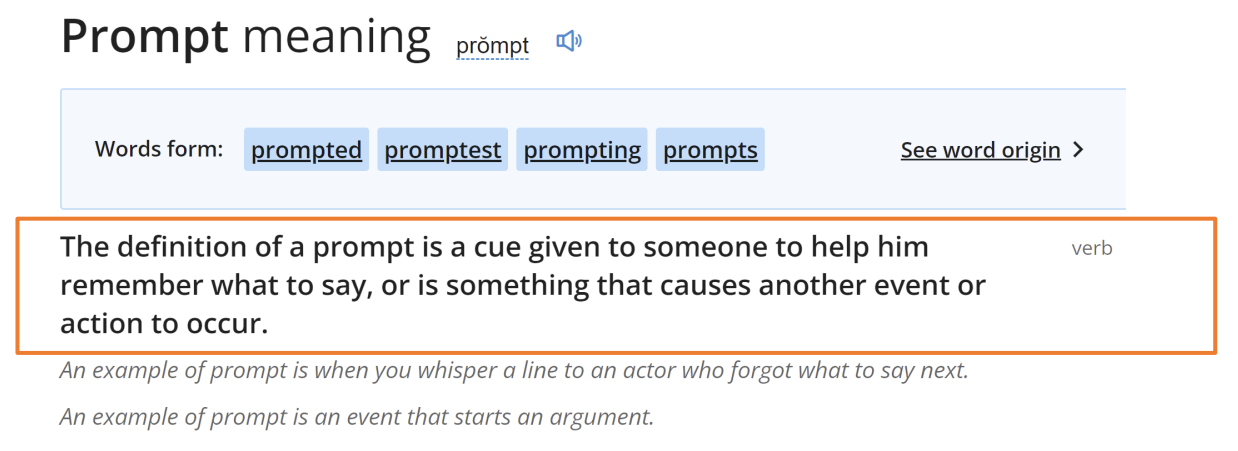
\includegraphics[width=\linewidth,keepaspectratio]{promptengg41}

{\tiny (Ref: The Fourth Paradigm of Modern Natural Language Processing Techniques - Pengfei Liu)}

\end{center}		

\end{frame}

%%%%%%%%%%%%%%%%%%%%%%%%%%%%%%%%%%%%%%%%%%%%%%%%%%%%%%%%%%%
\begin{frame}[fragile]\frametitle{Glorified Auto-complete?}


\begin{center}
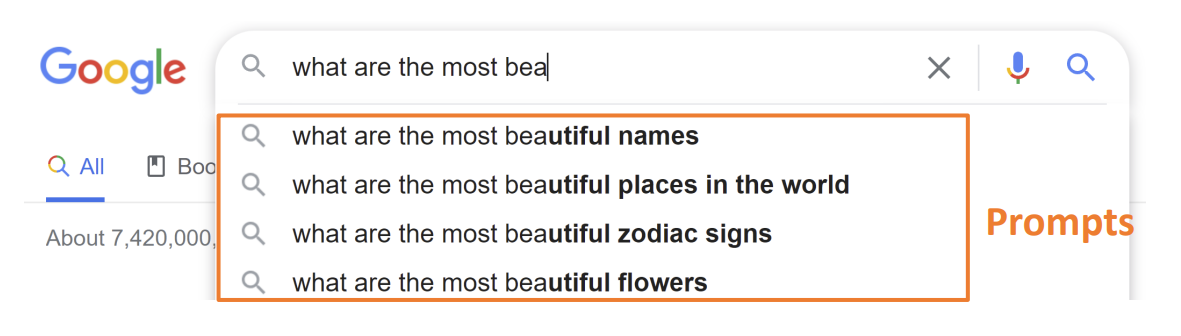
\includegraphics[width=\linewidth,keepaspectratio]{promptengg42}

{\tiny (Ref: The Fourth Paradigm of Modern Natural Language Processing Techniques - Pengfei Liu)}

\end{center}		

\end{frame}

%%%%%%%%%%%%%%%%%%%%%%%%%%%%%%%%%%%%%%%%%%%%%%%%%%%%%%%%%%%
\begin{frame}[fragile]\frametitle{What is a Prompt?}

\begin{itemize}
\item An Intuitive Definition: Prompt is a cue given to the pre-trained language model to allow it
better understand human’s questions
\item More Technical Definition: Prompt is the technique of making better use of the knowledge from
the pre-trained model by adding additional texts to the input.
\item Purpose: making better use of the knowledge
\item Method: adding additional texts to the input
\end{itemize}
\end{frame}

%%%%%%%%%%%%%%%%%%%%%%%%%%%%%%%%%%%%%%%%%%%%%%%%%%%%%%%%%%%
\begin{frame}[fragile]\frametitle{What is a Prompt?}


\begin{columns}
    \begin{column}[T]{0.6\linewidth}
		\begin{center}
		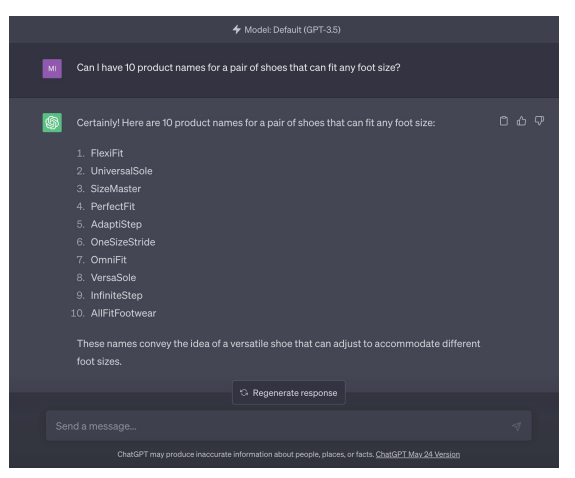
\includegraphics[width=\linewidth,keepaspectratio]{promptengg55}

		{\tiny (Ref: The Complete Prompt Engineering for AI Bootcamp (2023))}
		\end{center}	
    \end{column}
    \begin{column}[T]{0.4\linewidth}
		A prompt is the text we input to AI models when interfacing with them.
    \end{column}
  \end{columns}
\end{frame}



%%%%%%%%%%%%%%%%%%%%%%%%%%%%%%%%%%%%%%%%%%%%%%%%%%%%%%%%%%%
\begin{frame}[fragile]\frametitle{What is a Prompt?}
\begin{columns}
    \begin{column}[T]{0.6\linewidth}
		\begin{center}
		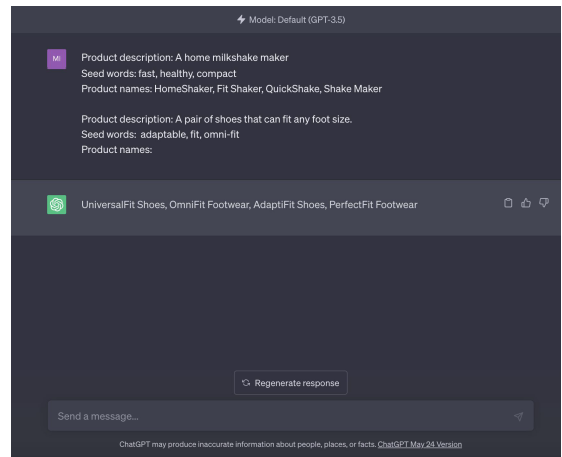
\includegraphics[width=\linewidth,keepaspectratio]{promptengg56}

		{\tiny (Ref: The Complete Prompt Engineering for AI Bootcamp (2023))}
		\end{center}	
    \end{column}
    \begin{column}[T]{0.4\linewidth}
		Prompt engineering is the process of discovering prompts which reliably yield useful or desired results.
    \end{column}
  \end{columns}
\end{frame}

%%%%%%%%%%%%%%%%%%%%%%%%%%%%%%%%%%%%%%%%%%%%%%%%%%%%%%%%%%%
\begin{frame}[fragile]\frametitle{What is Prompt Engineering?}

Prompt engineering is a NLP concept that involves discovering inputs that yield desirable or useful results


\begin{center}
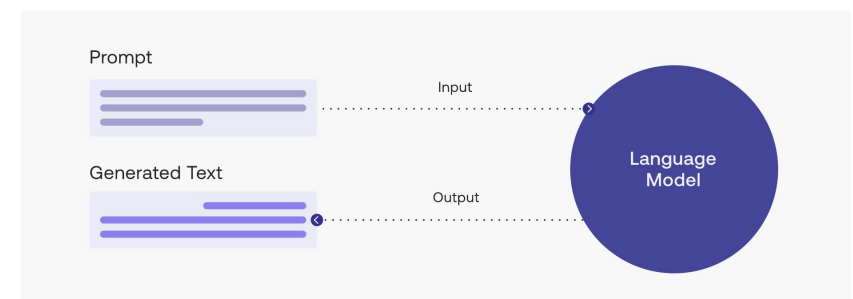
\includegraphics[width=\linewidth,keepaspectratio]{promptengg2}

{\tiny (Ref: Cohere https://docs.cohere.ai/docs/prompt-engineering)}

\end{center}				
\end{frame}

%%%%%%%%%%%%%%%%%%%%%%%%%%%%%%%%%%%%%%%%%%%%%%%%%%%%%%%%%%%
\begin{frame}[fragile]\frametitle{Why Prompt Engineering?}

\begin{itemize}
\item Important for research, discoveries, and advancement
\item Helps to test and evaluate the limitations of Large Language Models (LLMs)
\item Enables all kinds of innovative  applications on top of LLMs
\end{itemize}	

{\tiny (Ref: Prompt Engineering A lecture by DAIR.AI)}
\end{frame}



%%%%%%%%%%%%%%%%%%%%%%%%%%%%%%%%%%%%%%%%%%%%%%%%%%%%%%%%%%%
\begin{frame}[fragile]\frametitle{What is a Language Models?}

\begin{itemize}
\item While typing SMS, have you seen it suggests next word?
\item While typing email, have you seen next few words are suggested?
\item How does it suggest? (suggestions are not random, right?)
\item In the past, for ``Lets go for a \ldots', if you have typed 'coffee' 15 times, 'movie' say 4 times, then it learns that. Machine/Statistical Learning.
\item Next time, when you type ``Lets go for a '', what will be suggested? why?
\item This is called Language Model. Predicting the next word. When done continuously, one after other, it spits sentence, called Generative Model.
\end{itemize}	

\begin{center}
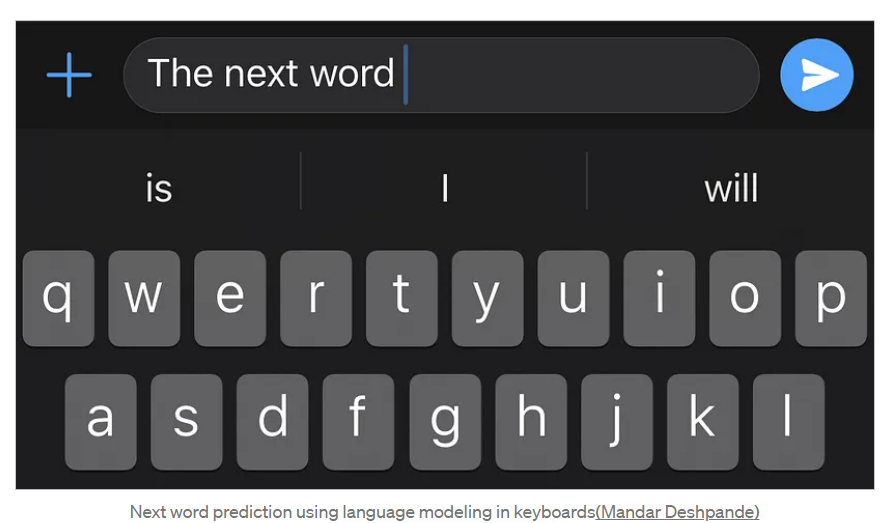
\includegraphics[width=0.6\linewidth,keepaspectratio]{chatgpt34}
\end{center}		

\end{frame}

%%%%%%%%%%%%%%%%%%%%%%%%%%%%%%%%%%%%%%%%%%%%%%%%%%%%%%%%%%%
\begin{frame}[fragile]\frametitle{Evolution of Language Models}

Language Models can be statistical (frequency based) or Machine/Deep Learning (supervised) based. Simple to complex.

\begin{center}
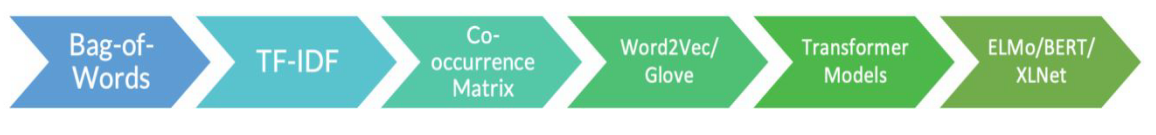
\includegraphics[width=\linewidth,keepaspectratio]{chatgpt30}
\end{center}				
{\tiny (Ref: Analytics Vidhya https://editor.analyticsvidhya.com/uploads/59483evolution\_of\_NLP.png)}

\end{frame}

%%%%%%%%%%%%%%%%%%%%%%%%%%%%%%%%%%%%%%%%%%%%%%%%%%%%%%%%%%%
\begin{frame}[fragile]\frametitle{Large Language Models - Comparison}

\begin{center}
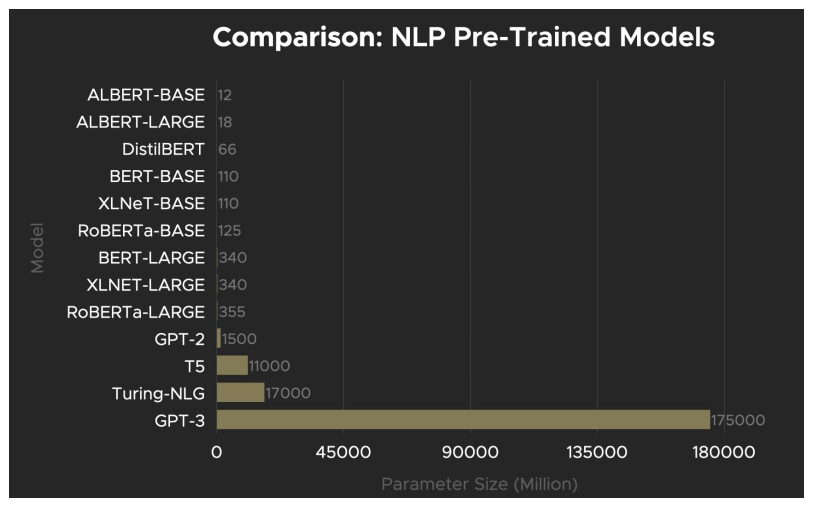
\includegraphics[width=\linewidth,keepaspectratio]{chatgpt31}
\end{center}				
{\tiny (Ref: Deus.ai https://www.deus.ai/post/gpt-3-what-is-all-the-excitement-about)}

\end{frame}

%%%%%%%%%%%%%%%%%%%%%%%%%%%%%%%%%%%%%%%%%%%%%%%%%%%%%%%%%%%
\begin{frame}[fragile]\frametitle{Progression}

Models for prediction:

\begin{itemize}
\item On data, derive features, put statistical techniques like regression. One model per task. That's Machine Learning.
\item Feed raw data, employ neural networks. One model per task. That's Deep Learning.
\item Use Text data, get embeddings, use ML/DL, say for classification. One model per task. That's Natural Language Processing.
\item Train neural network on large corpus, store weights and architecture, then add final layers for say classification on custom data+labels. That's Pretrained model. One model, many tasks.
\item Train Large Language Model, just supply instructions on what to do, works. One model many tasks. Zero-shot, few-shots.
\end{itemize}

{\tiny (More info at SaaS LLM https://medium.com/google-developer-experts/saasgpt-84ba80265d0f)}

\end{frame}



%%%%%%%%%%%%%%%%%%%%%%%%%%%%%%%%%%%%%%%%%%%%%%%%%%%%%%%%%%%
\begin{frame}[fragile]\frametitle{Pace of AI Innovation}

\begin{center}
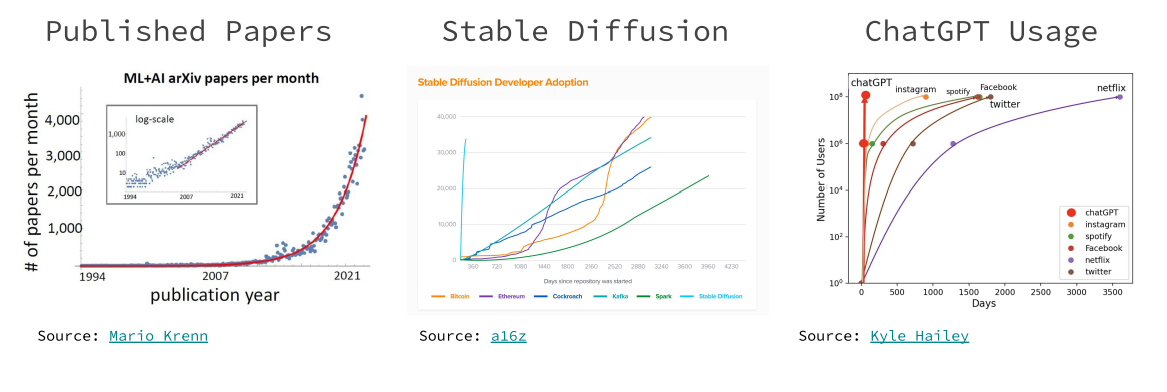
\includegraphics[width=\linewidth,keepaspectratio]{promptengg57}

{\tiny (Ref: The Complete Prompt Engineering for AI Bootcamp (2023))}

\end{center}

Stable Diffusion: see the blue line, almost Y axis.
				
\end{frame}

%%%%%%%%%%%%%%%%%%%%%%%%%%%%%%%%%%%%%%%%%%%%%%%%%%%%%%%%%%%
\begin{frame}[fragile]\frametitle{Prompt Engineering Interest}

\begin{center}
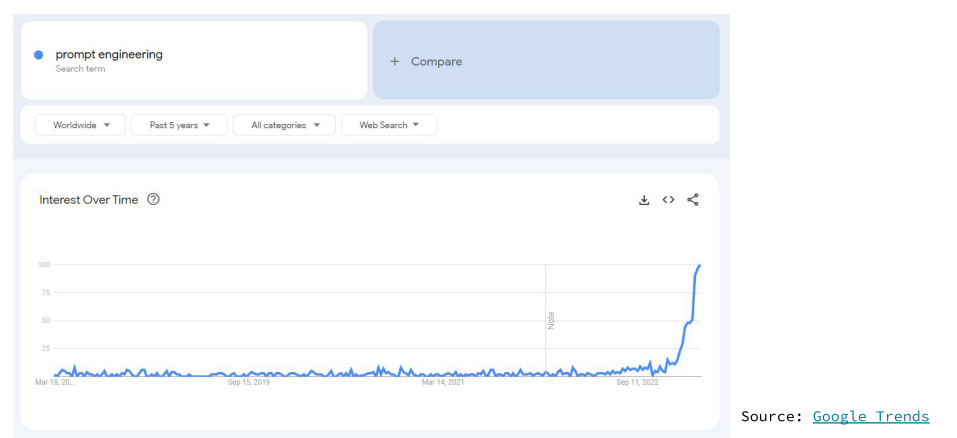
\includegraphics[width=\linewidth,keepaspectratio]{promptengg58}

{\tiny (Ref: The Complete Prompt Engineering for AI Bootcamp (2023))}

\end{center}		

Skill for everyone, just like Google Search.
		
\end{frame}

%%%%%%%%%%%%%%%%%%%%%%%%%%%%%%%%%%%%%%%%%%%%%%%%%%%%%%%%%%%
\begin{frame}[fragile]\frametitle{Why Learn Prompt Engineering?}

Avoid Inconsistent Results

\begin{center}
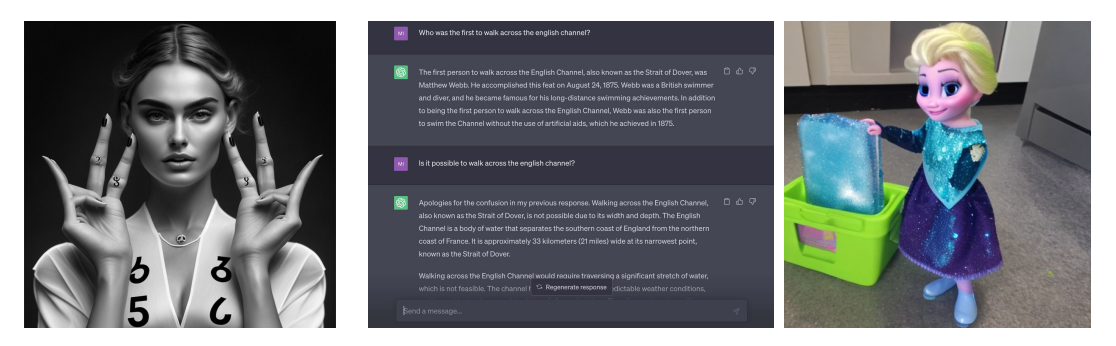
\includegraphics[width=\linewidth,keepaspectratio]{promptengg59}

{\tiny (Ref: The Complete Prompt Engineering for AI Bootcamp (2023))}

\end{center}	


Avoiding Hallucination, making it more precise. Image with no arms?
			
\end{frame}

%%%%%%%%%%%%%%%%%%%%%%%%%%%%%%%%%%%%%%%%%%%%%%%%%%%%%%%%%%%
\begin{frame}[fragile]\frametitle{Why Learn Prompt Engineering?}

Use Advanced Techniques

\begin{center}
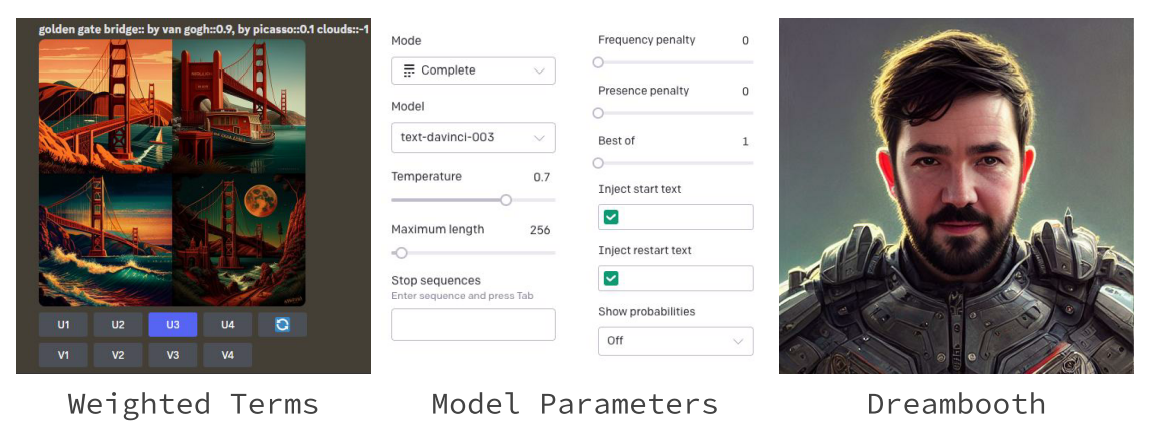
\includegraphics[width=\linewidth,keepaspectratio]{promptengg60}

{\tiny (Ref: The Complete Prompt Engineering for AI Bootcamp (2023))}
\end{center}	

Mixing styles, Picasso + Van Gogh. 
Dreambooth make your own Avatar.
			
\end{frame}

%%%%%%%%%%%%%%%%%%%%%%%%%%%%%%%%%%%%%%%%%%%%%%%%%%%%%%%%%%%
\begin{frame}[fragile]\frametitle{Why Learn Prompt Engineering?}

Scale Creative Output

\begin{center}
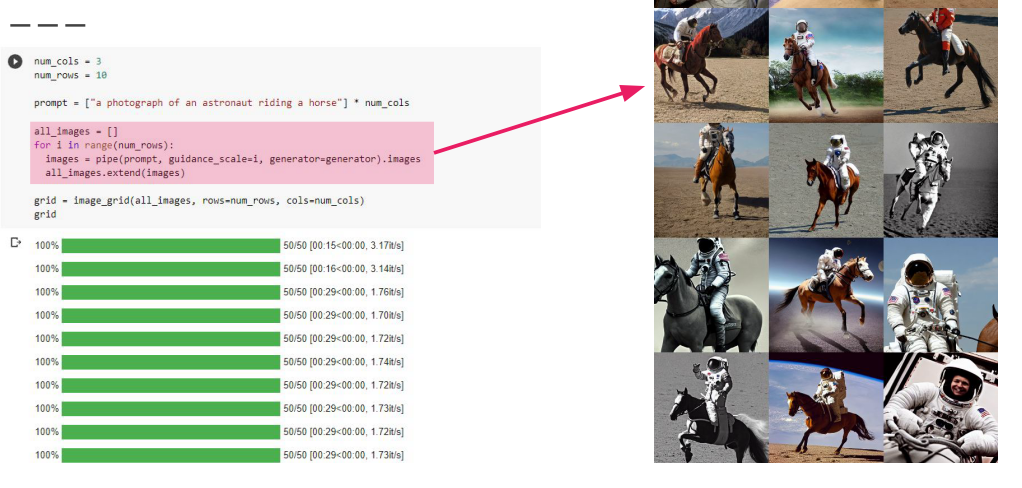
\includegraphics[width=\linewidth,keepaspectratio]{promptengg61}

{\tiny (Ref: The Complete Prompt Engineering for AI Bootcamp (2023))}
\end{center}	

Create different variations, programmatically.
			
\end{frame}


